\documentclass[11pt,oneside]{amsart}
\usepackage{geometry}                % See geometry.pdf to learn the layout options. There are lots.
\geometry{a4paper}                   % ... or a4paper or a5paper or ... 
%\geometry{landscape}                % Activate for for rotated page geometry
\usepackage[parfill]{parskip}    % Activate to begin paragraphs with an empty line rather than an indent
\usepackage{xcolor}
\usepackage{graphicx}
\usepackage{amssymb}
\usepackage{epstopdf}
\usepackage{algorithm}
\usepackage{algorithmic}
\usepackage{subcaption}

\usepackage{sidecap}
\usepackage{hyperref}
\usepackage{xspace}
\usepackage{tcolorbox}
\DeclareGraphicsRule{.tif}{png}{.png}{`convert #1 `dirname #1`/`basename #1 .tif`.png}
\renewcommand{\baselinestretch}{1.2}

\usepackage{biblatex}
\addbibresource{references.bib}

%%%% Some handy commands
\newcommand{\Acc}{\mathcal A}
\newcommand{\Op}{\hat{\mathcal O}}
\newcommand{\bL}{\hat L}
\newcommand{\Cl}{Cl$^-$\xspace}
\newcommand{\HCO}{HCO$_3$\xspace}
\newcommand{\gabar}{GABA$_A$R\xspace}




%%%%%%%%%%%%%%%%%%%%%%%%%%%%%%%%%%%%%%%%%%%%%%%%%%%%%%%%%%%%%%%%%%%%%%
%%%%%%%%%%%%%%%%%%%%%%%%%%%%%%%%%%%%%%%%%%%%%%%%%%%%%%%%%%%%%%%%%%%%%%
\title[NE TN0180]{Where do PSPs come from? \\  NE TN0810}
\author{G. Ruffini}
%\date{\today}           % Activate to display a given date or no date

%%%%%%%%%%%%%%%%%%%%%%%%%%%%%%%%%%%%%%%%%%%%%%%%%%%%%%%%%     %%%%%%%%%%%%%
\begin{document}
\maketitle

\begin{abstract}
\normalsize
    Why do post-synaptic potentials (PSPs) have the shape they do? 
Sometimes PSPs are modeled by the impulse response with an exponential shape. Where does this come from?

The physics are governed by the cable and synapse kinetic equations, and the mathematics by the theory of linear differential equations, and more specifically their impulse response. 

We describe the transformation ladder from an idealized delta function action potential to the dynamics of conductance, synaptic current, voltage or chlorine concentration.

We show where the single and double exponential functions come from from a few assumptions. We discuss the possibility of simplification for the case of chlorine accumulation. 

\end{abstract}

%\usepackage{}\clearpage
\tableofcontents


\clearpage
%%%%%%%%%%%%%%%%%%%%%%%%%%%%%%%%%%%%%%%%%%%%%%%%%%%%%%%%%%%%%%%%%%%%%%
\section{Introduction}
\label{sec:introduction}
The reader may have wondered where the typical expression for PSP  comes from, or, equivalently, the "L" operator or h-box.  Here I try to explain from the analysis of the sequence of events from an action potential generated release of a neurotransmitter. To simplify this, I will assume that the action potential itself can be represented by a delta function. This is definitely an approximation, I could use some more realistic pulse shape, but we can revisit this at the end. The point is that it is assume to be a sharp event, with a time scale shorter than that of the ones involved downstream, 
\begin{equation}
A(t) = \delta(t)
\end{equation}

A word about linear differential operators: linear ODEs can be written down in the form
$$
L[x(t)] = (\frac{d}{dt} -\lambda_1)(\frac{d}{dt} -\lambda_2)...(\frac{d}{dt} -\lambda_n)
$$
The general solution to the homogeneous problem $L[x_h(t)]=0$ if all the $\lambda$s are different, is 
$$
x_h(t) = \sum c_i e^{\lambda_i t}
$$
The solution to the impulse problem, $L[x_i(t)] = \delta(t)$ is of the form
$$
x_i(t) = H(t)\sum c_i e^{\lambda_i t}
$$
To see this, note that to the left of the discontinuity at $t=0$, the solution should be zero, and to the right, it should be a homogeneous solution. To fix the constants in the latter, the BCs we use is that all all the derivatives of $x_i(t)$ should be zero at $t=0$ (continuity) except the one before last ($x^{(n-1)}(t)=1$), which should reflect a step discontinuity. 

Camporesi gives and expression for the general formula \cite{camporesi11}.

%%%%%%%%%%%%%%%%%%%%%%%%%%%%5
\section{Transforming the action potential into a conductance change and synaptic current}

What happens next? Fist the action potential is transformed into the influx of some ionic species into the cell. This transforms the shape of the action potential signal, low-pass filtering  it. This is governed by the dynamics of conductance $z(t)$. The underlying equation is
\begin{equation}
I_s = \bar g \, (V-V_R)\,  z(t)
\end{equation}
The dynamics of conductance are governed by second order linear operator, which we can think of as describing the rise and decay times. 
$$
L_s[z(t)] = (\frac{d}{dt} + a_r)(\frac{d}{dt} +a_d) \, z(t)
$$

Therefore, the conductance and current dynamics from an impulsive action potential are (see G. Bard Ermentrout and David H. Terman section 71., Mathematical Foundations of Neuroscience),  
\begin{equation}
I_s(t) = \bar g \, (V-V_R)\,  z(t) = \bar g \, (V-V_R) \frac{a_d\, a_r}{a_r-a_d}(e^{-a_dt}-e^{-a_rt} )\,  H(t)
\end{equation}
where we assume the membrane voltage and reversal potential are minimally affected during this process (they are slowly varying).


%%%%%%%%%%%%%%%%%%%%%%%%%%%%%%%%%%%%%%%%%%%%%%%%%%%%%%%%%%%%%%%%%%%%%%
\section{From action potential to current to voltage}
\label{sec:input}

The next step down the ladder is to solve the equation for voltage perturbation $u(t)$. 
The equation here is the single compartment cable equation. 
In simplified form, for a single compartment conservation of current dictates the following first order differential equation,
$$C_m \frac{\partial V}{\partial t} + \frac{V}{R_m}= I_s$$
The impulse response of this (ie, when $I_s$ is a delta function) is an exponential function, characterized by $\tau = C_m  R_m$. 

%%%%%%%%%%%%%%%%%%%%%%%5
\begin{figure}[t!]
    \centering
    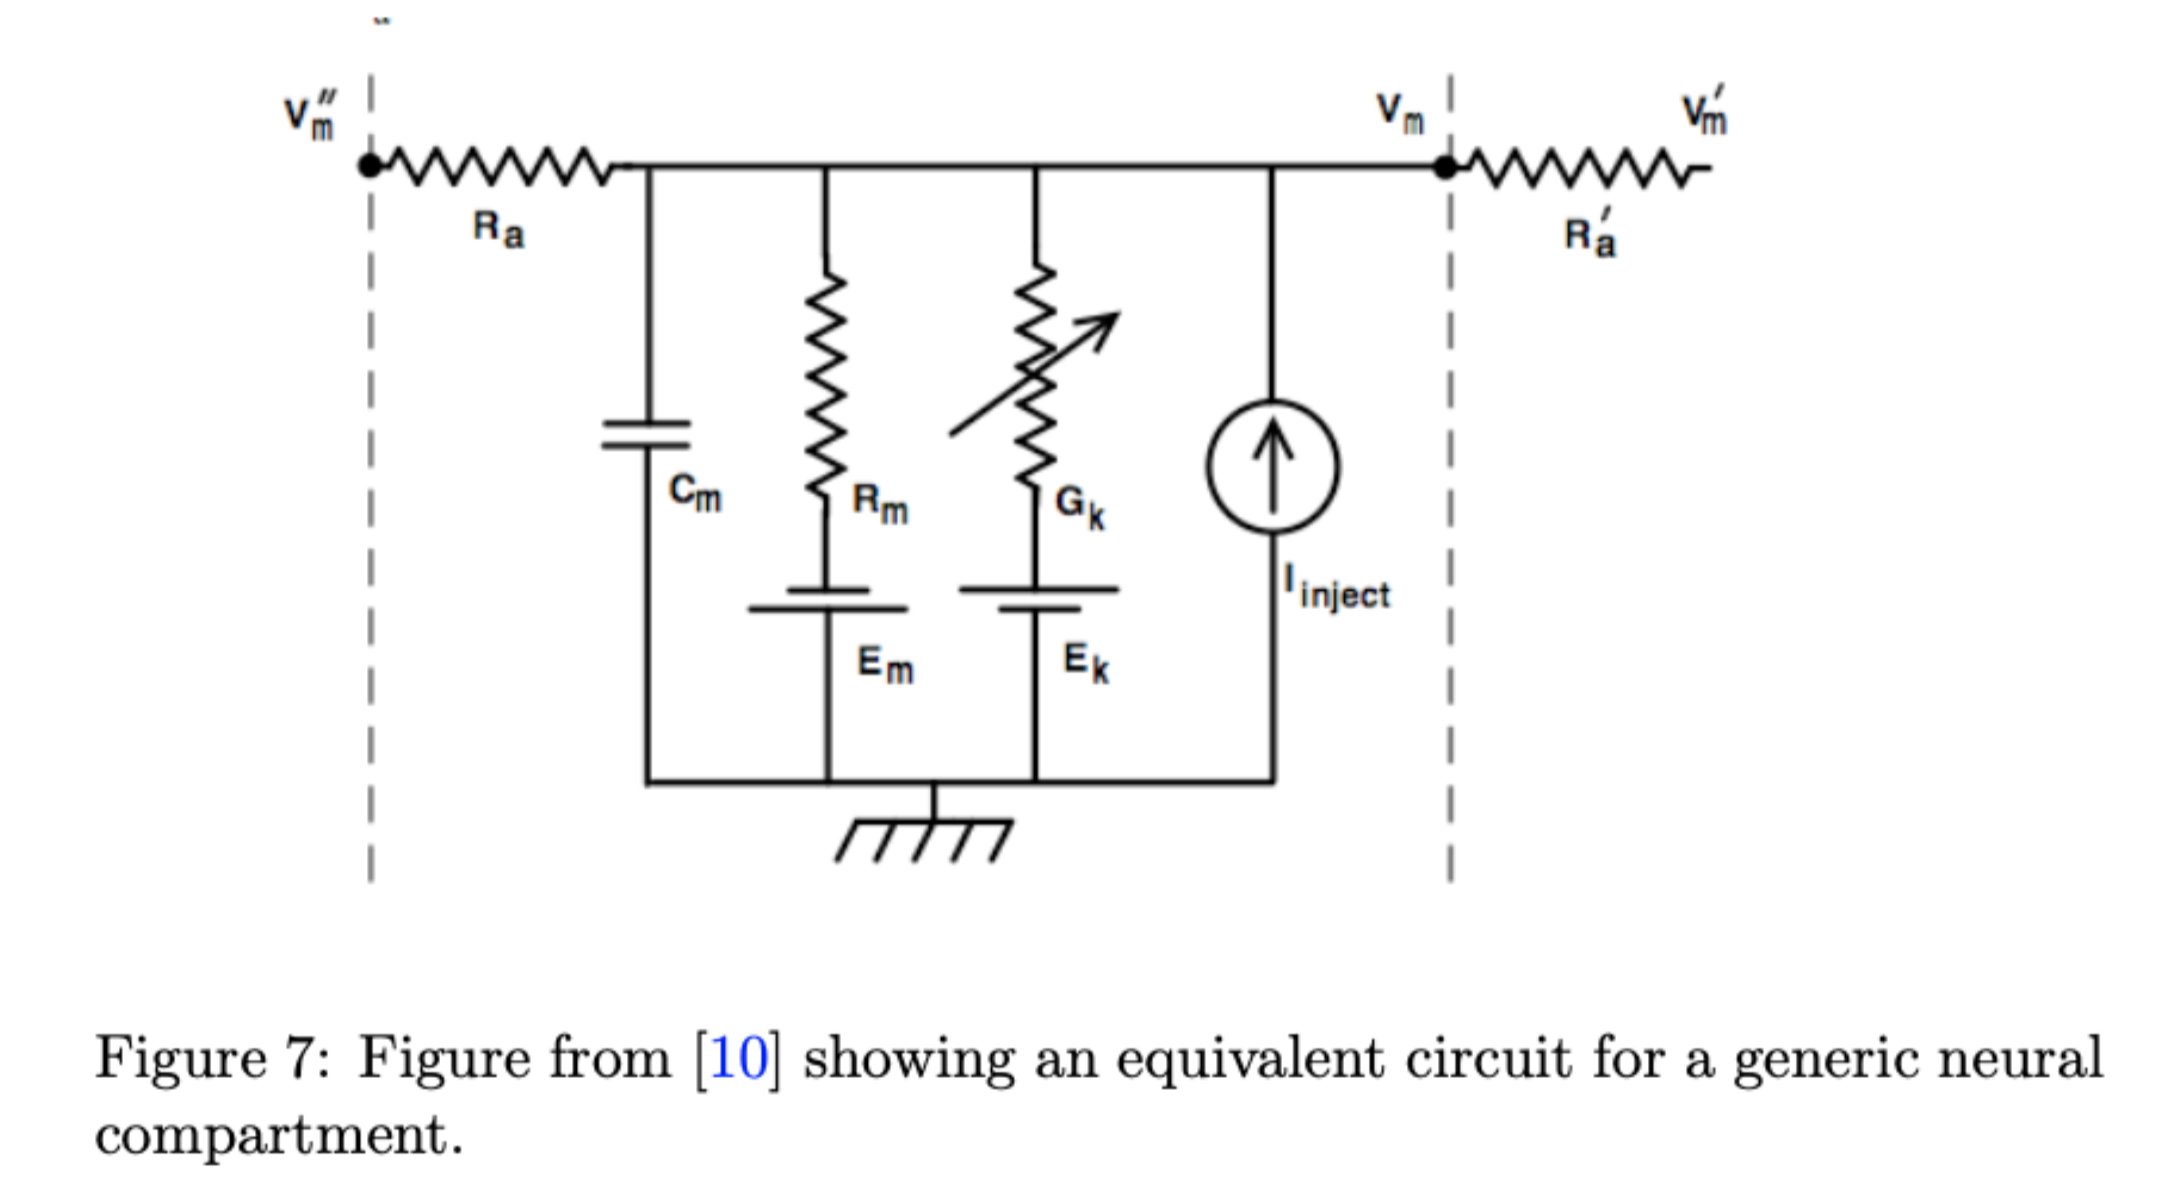
\includegraphics[width=9.5cm]{figures/bower.png}
    \caption{{\bf Equivalent circuit for single compartment with dynamic conductance (From Bower/Genesis.}}
    \label{fig:linear}
\end{figure}
%%%%%%%%%%%%%%%%%%%%%%%%%%%



Thus, this is of the form
\begin{equation}
L_m[u_i(t)]=I_s(t)
\end{equation}
with $L_m = (\frac{d}{dt} +a_m)$, a first order operation with $a_m =1/R_mC_m$ (membrane resistivity and capacitance),  or, since $L_s[I_s(t)]= \bar g(V-V_R) \delta(t) $
 \begin{equation}
L_s[L_m[u_i(t)]]=\bar g(V-V_R)  \, \delta(t)
\end{equation}
The impulse response is now of the form
\begin{equation}
    u_i(t) = A\, \bar g(V-V_R) (c_d e^{-a_rt}+ c_r e^{-a_dt} +c_m e^{-a_mt})\, H(t) 
\end{equation}
Note that here we ignored the fact that $V$ is a function of time. It is assumed to vary slowly, with a small perturbation proportional to $u$, i.e., $V(t)=V_s(t)+u(t)$ with $V_0(s)-V_R>>u(t)$, and with $V_s(t)$ a slowly varying quantity compared to the time constants at hand (i.e., $1/a_m$). 

If one of the time constants is very small compared to the others, it will not play much of a role once the impulse is used in a convolution. This is not very clearly the case here, because the electrical time constant may also be very small in neurites and such. 

However, another simplification may be warranted if one of the time constants is between the other two. Although the precise form of the PSP depends on it, its impact is less obvious than that of the other two, which determine rise time and fall time.


A simple tradeoff may be to only take the smallest and largest time constant. This leads to the usual double exponential form for PSPs, 
\begin{equation}
    u_i(t)= H(t)\frac{a_ra_m}{a_r-a_m} ( e^{-a_r t}-  e^{-a_mt})
\end{equation}
If we assume that the two roots are equivalent ($a_r =a_m$), then the solution of the ODE is a bit different, 
\begin{equation}
    u_i(t)= H(t) \, t e^{-a t}
\end{equation}


%%%%%%%%%%%%%%%%%%%%%%%5
\begin{figure}[t!]
    \centering
    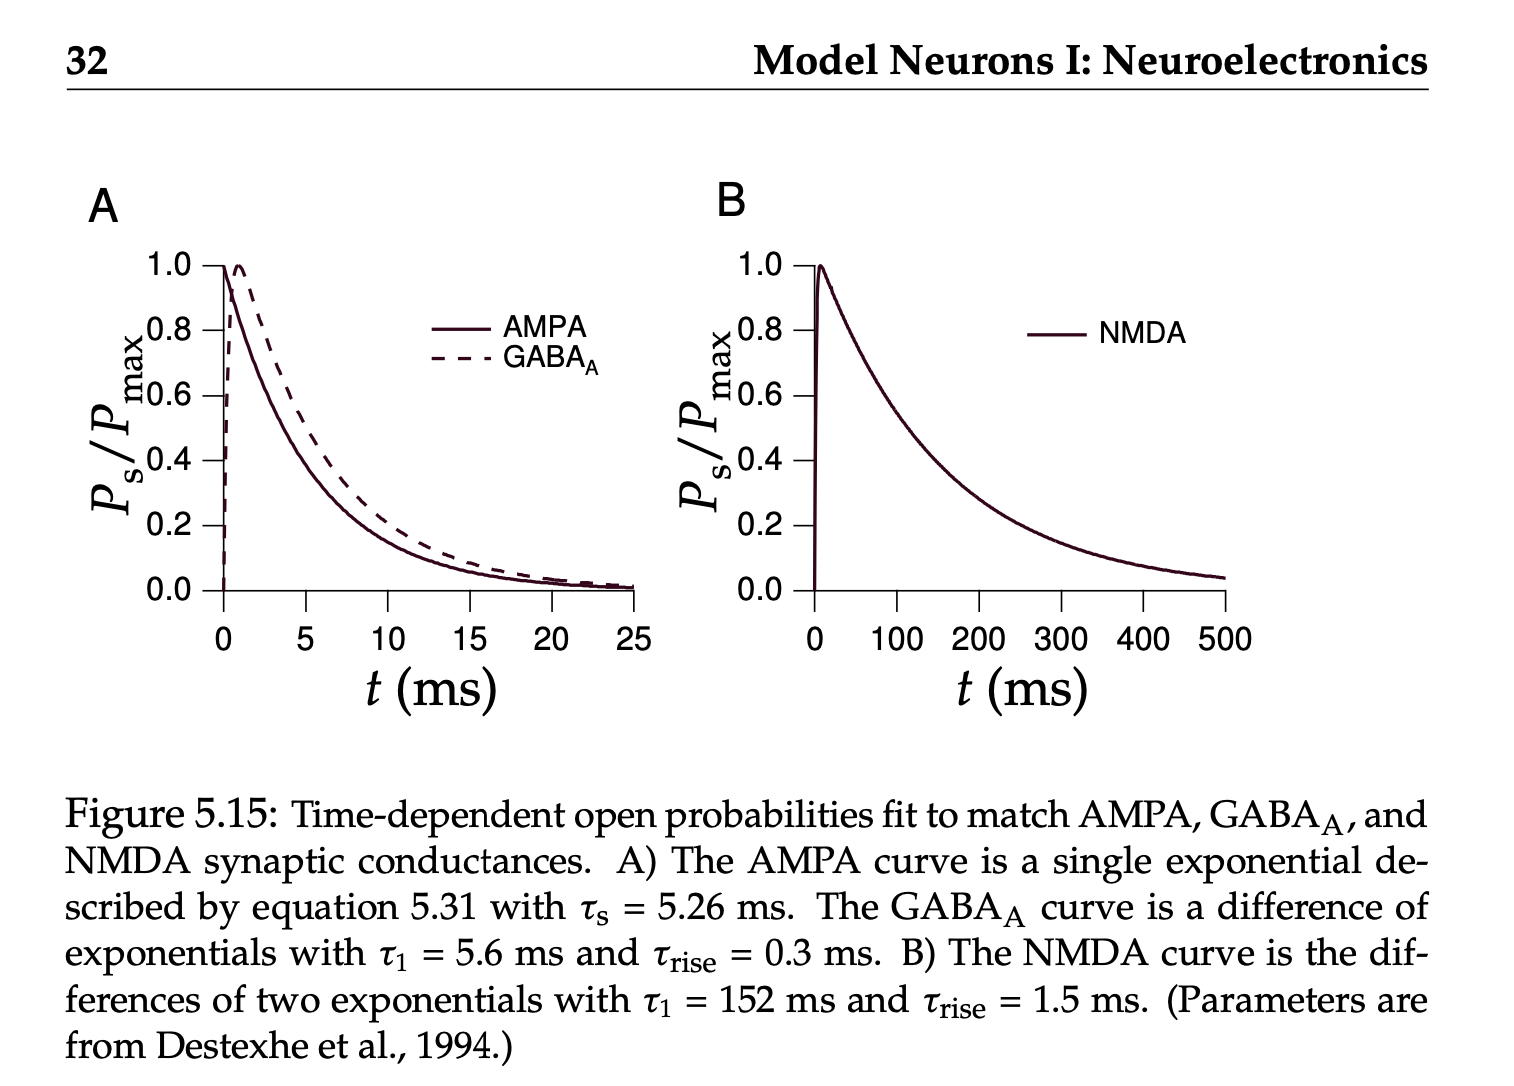
\includegraphics[width=9.5cm]{figures/conductances.png}
    \caption{{\bf Conductance dynamics (From Bower/Genesis.}}
    \label{fig:linear}
\end{figure}
%%%%%%%%%%%%%%%%%%%%%%%%%%%
%%%%%%%%%%%%%%%%%%%%%%%%%%%%%%%%%%%%%%%%%%%%%%%%%%%%%%%%%%%%%%%%%%%%%%
\section{From current to {[$\mbox{Cl}^-$]} }
Let us first express the firing rate as a function of action potentials.
The action potential time series is of the form
$$
A(t) = \sum_n \delta(t-t_n) 
$$
and the firing rate is a running average of this over some time window $\Delta t$, which we write as 
$$
\varphi(t) = \langle A(t') \rangle_t  = 
 \frac{ 1}{\Delta T} \int_t^{t+\Delta t} dt\,  A(t')  
$$

We actually need the analog of these in terms of synaptic flux, which is proportional to synaptic current. This is given by the flux conductance rate, 
$$
\tilde g(t)= L_s^{-1}[\varphi(t)] =  \frac{ k}{\Delta T} \int_t^{t+\Delta t} dt\,  L_s^{-1}[A(t')] 
$$

 Letting $\rho(t) = [\text {Cl}^{-}]_i$,
$$
\frac{d\rho}{dt} =  \alpha  L_s^{-1}[\varphi(t)] \ (E_{GABA}(t) - V_m) - \alpha_{KCC2} \left( E_{Cl^-}(t) -  E_{K^+} \right).
$$

The solution to the differential equation is given by
\begin{eqnarray*}
    \rho(t) &=& \rho_0 +
    \alpha \int_{t_0}^t dt'\,  L_s^{-1}[\varphi(t')] \ (E_{GABA}(t') - V_m) - \alpha_{KCC2} \int_{t_0}^t dt'\, \left( E_{Cl^-}(t') -  E_{K^+} \right)\\
    &=& \rho_0 +
    \alpha L_s^{-1}\left[\int_{t_0}^t dt'\,  \varphi(t') \ (E_{GABA}(t') - V_m) \right]- \alpha_{KCC2} \int_{t_0}^t dt'\, \left( E_{Cl^-}(t') -  E_{K^+} \right) \\
 &\approx&     \rho_0 +
    \alpha \int_{t_0}^t dt'\,  \varphi(t') \ (E_{GABA}(t') - V_m) - \alpha_{KCC2} \int_{t_0}^t dt'\, \left( E_{Cl^-}(t') -  E_{K^+} \right)
\end{eqnarray*}
Here $\rho_0$ refers to the baseline concentration at some initial time $t_0$. 

The last approximation refers to the fact that for $t \approx t_0$, the contribution of the integrals is small compared to the baseline concentration $\rho_0$. For bigger times, the effect of the integral is accumulation  the firing rate (i.e., total number of counts), which is a slowly varying function. In other words, the fast stuff (associated with firing rate changes) will not be important on the scale of big things. The firing rate will add some small ``ripples" to the history of concentration, but the argument is that these small ripples can be ignored for the purposes of computing derived quantities such as $E_{GABA}(\rho)$. Whether we low-pass filter them a bit or leave them unfiltered will not matter much to the end result.


%%%%%%%%%%%%%%%%%%%%%%%%%%%%%%%%%%%%%%%%%%%%%

\section{Conclusions}
 We provide a unified picture of the mechanisms liking action potentials idealized by a Dirac delta function with conductance, synaptic current and then potential and chlorine accumulation. In particular, we provide a rationale for the usual expression for PSPs using one or two exponential functions, and for simplifying the picture to one exponential for the chlorine transport. This means we can ignore the synaptic L operator in that case, taking care only of units.
 

 
\printbibliography

\end{document}  
